\chapter{Introduction}
\label{chap:Intro}


\section{Motivation}

Since the discovery of the laser \cite{schawlowInfraredOpticalMasers1958, maimanStimulatedOpticalRadiation1960}, and the subsequent demonstration of nonlinear optics \cite{frankenGenerationOpticalHarmonics1961}

\begin{figure}
	\centering
	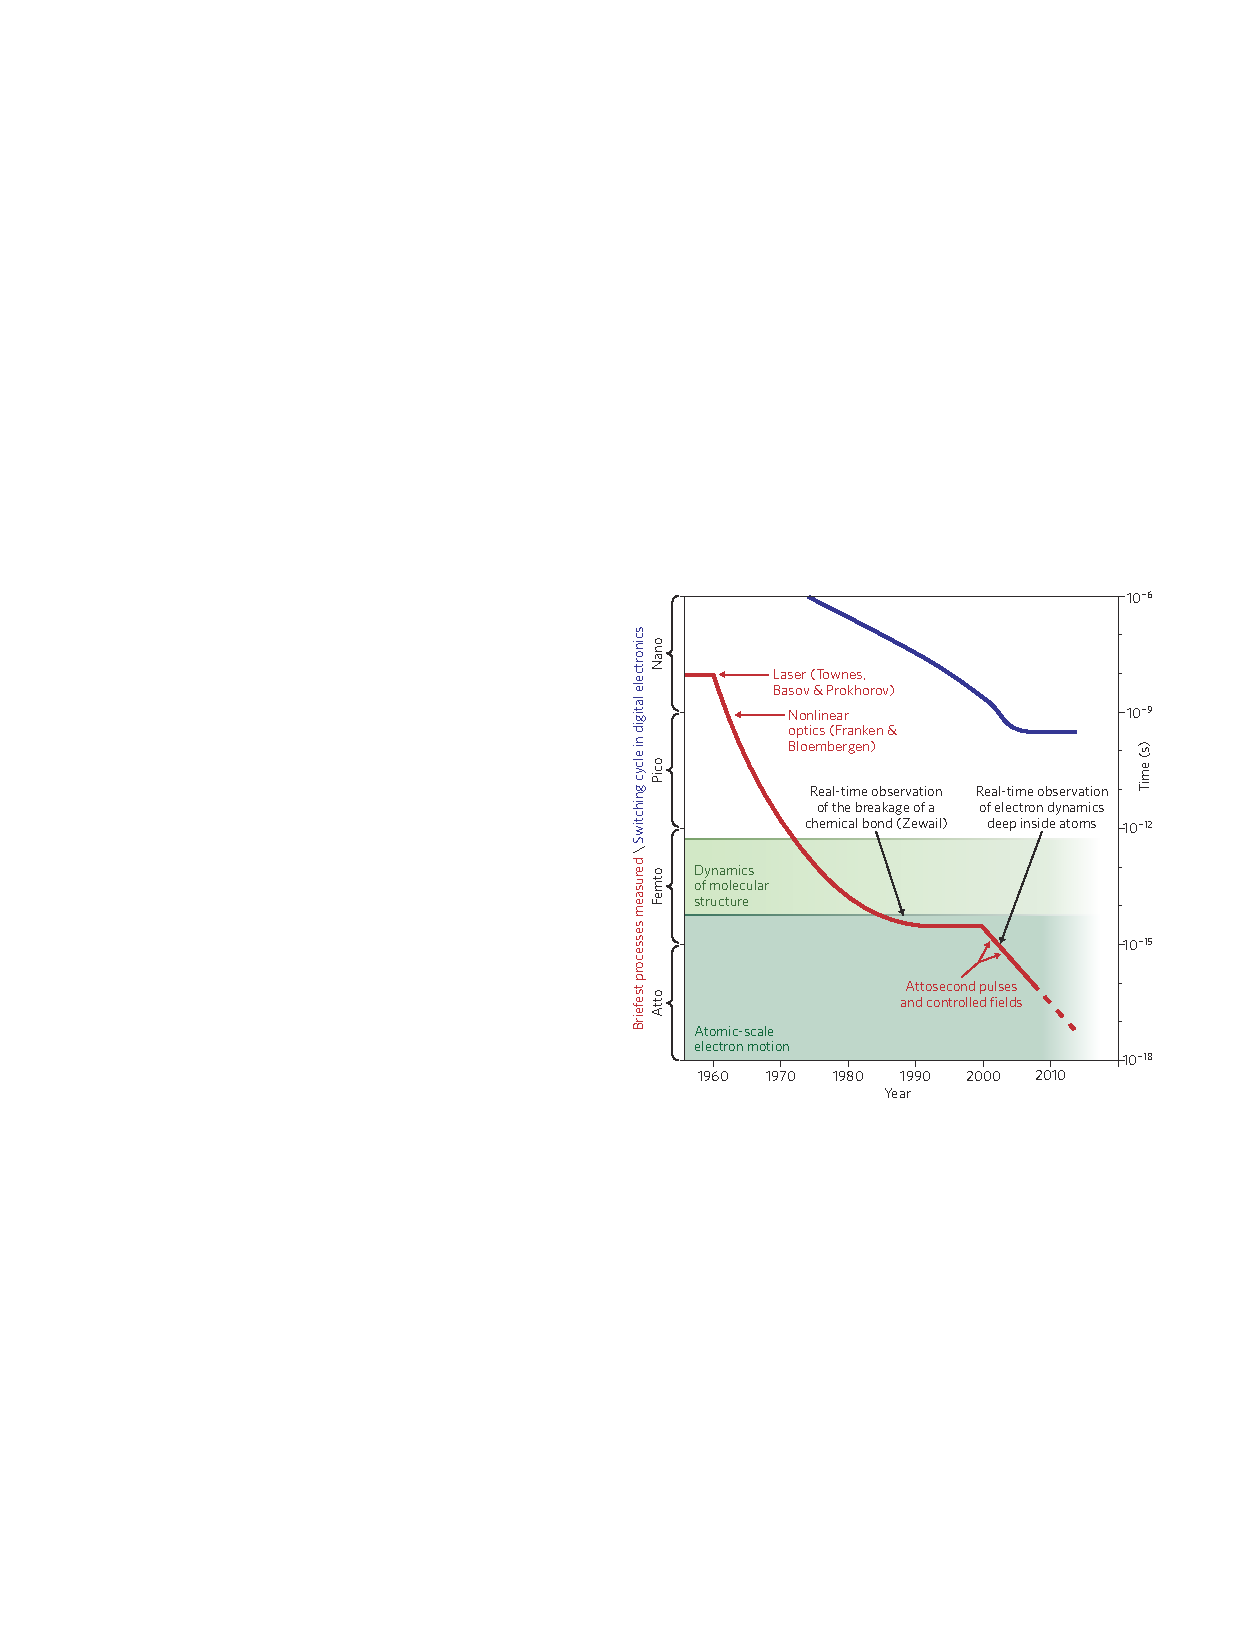
\includegraphics[width=0.5\textwidth]{figures/Introduction/Pulse_duration.pdf}
	\caption[Recollision model of high harmonic generation]{Recollision model of high harmonic generation.  The three steps are (1) tunnel ionization, (2) propagation/accelaration in the laser field, and (3) recombination and photoemission.}
	\label{fig:pulse_duartion}
\end{figure}

\section{HHG and APT}
\label{intro_HHG}

\begin{figure}
	\centering
	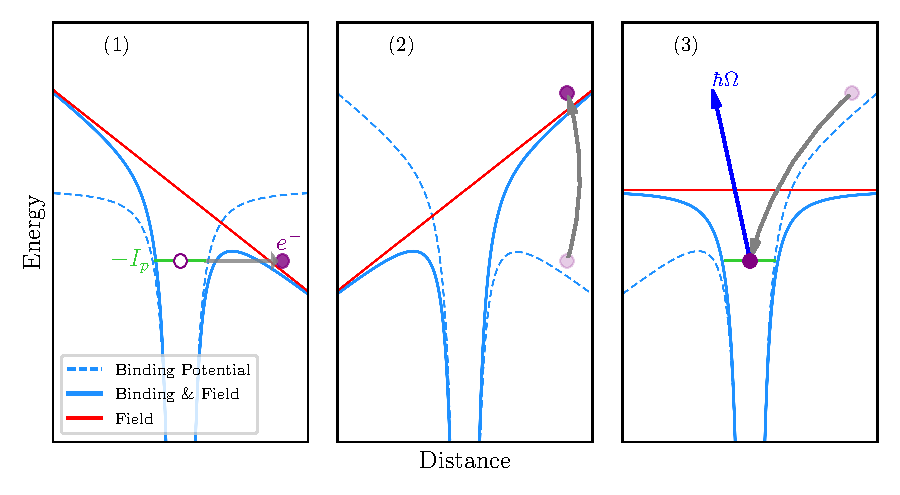
\includegraphics[width=0.9\textwidth]{figures/Introduction/3-step.pdf}
	\caption[Recollision model of high harmonic generation]{Recollision model of high harmonic generation.  The three steps are (1) tunnel ionization, (2) propagation/accelaration in the laser field, and (3) recombination and photoemission.}
	\label{fig:3-step}
\end{figure}

\begin{figure}
	\centering
	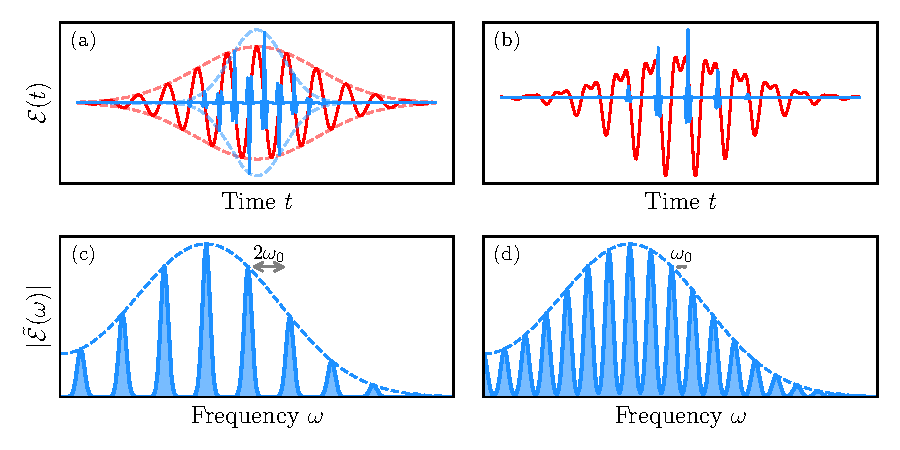
\includegraphics[width=1.0\textwidth]{figures/Introduction/time_to_freq.pdf}
	\caption[Example electric field of XUV APT and its frequency spectrum]{(a) Example of the electric field of an XUV APT.  There is a burst every half-cycle of the fundamental field period $\tau_0$.  (b)  Spectral amplitude of APT.  Harmonics are separated by $2\omega_0=4\pi/\tau_0$.  Bandwidth of each harmonic is determined by the number of cycles in the fundamental pulse, and the overall bandwidth is determined by the pulse duration of each burst in the train. (b) Example of a two-color $\omega-2\omega$ fundamental field.  The asymmetry of the pulse means there is a burst once every cycle. (d) The spectral amplitude for the asymmetric field, and now there are even and odd harmonics.  The dashed line in (c) and (d) represent the spectral amplitude of just one of the pulses in the pulse train.}
	\label{fig:time_to_freq}
\end{figure}


\section{CATS: real and imaginary}
\label{into_theory_cats}

\begin{figure}
	\centering
	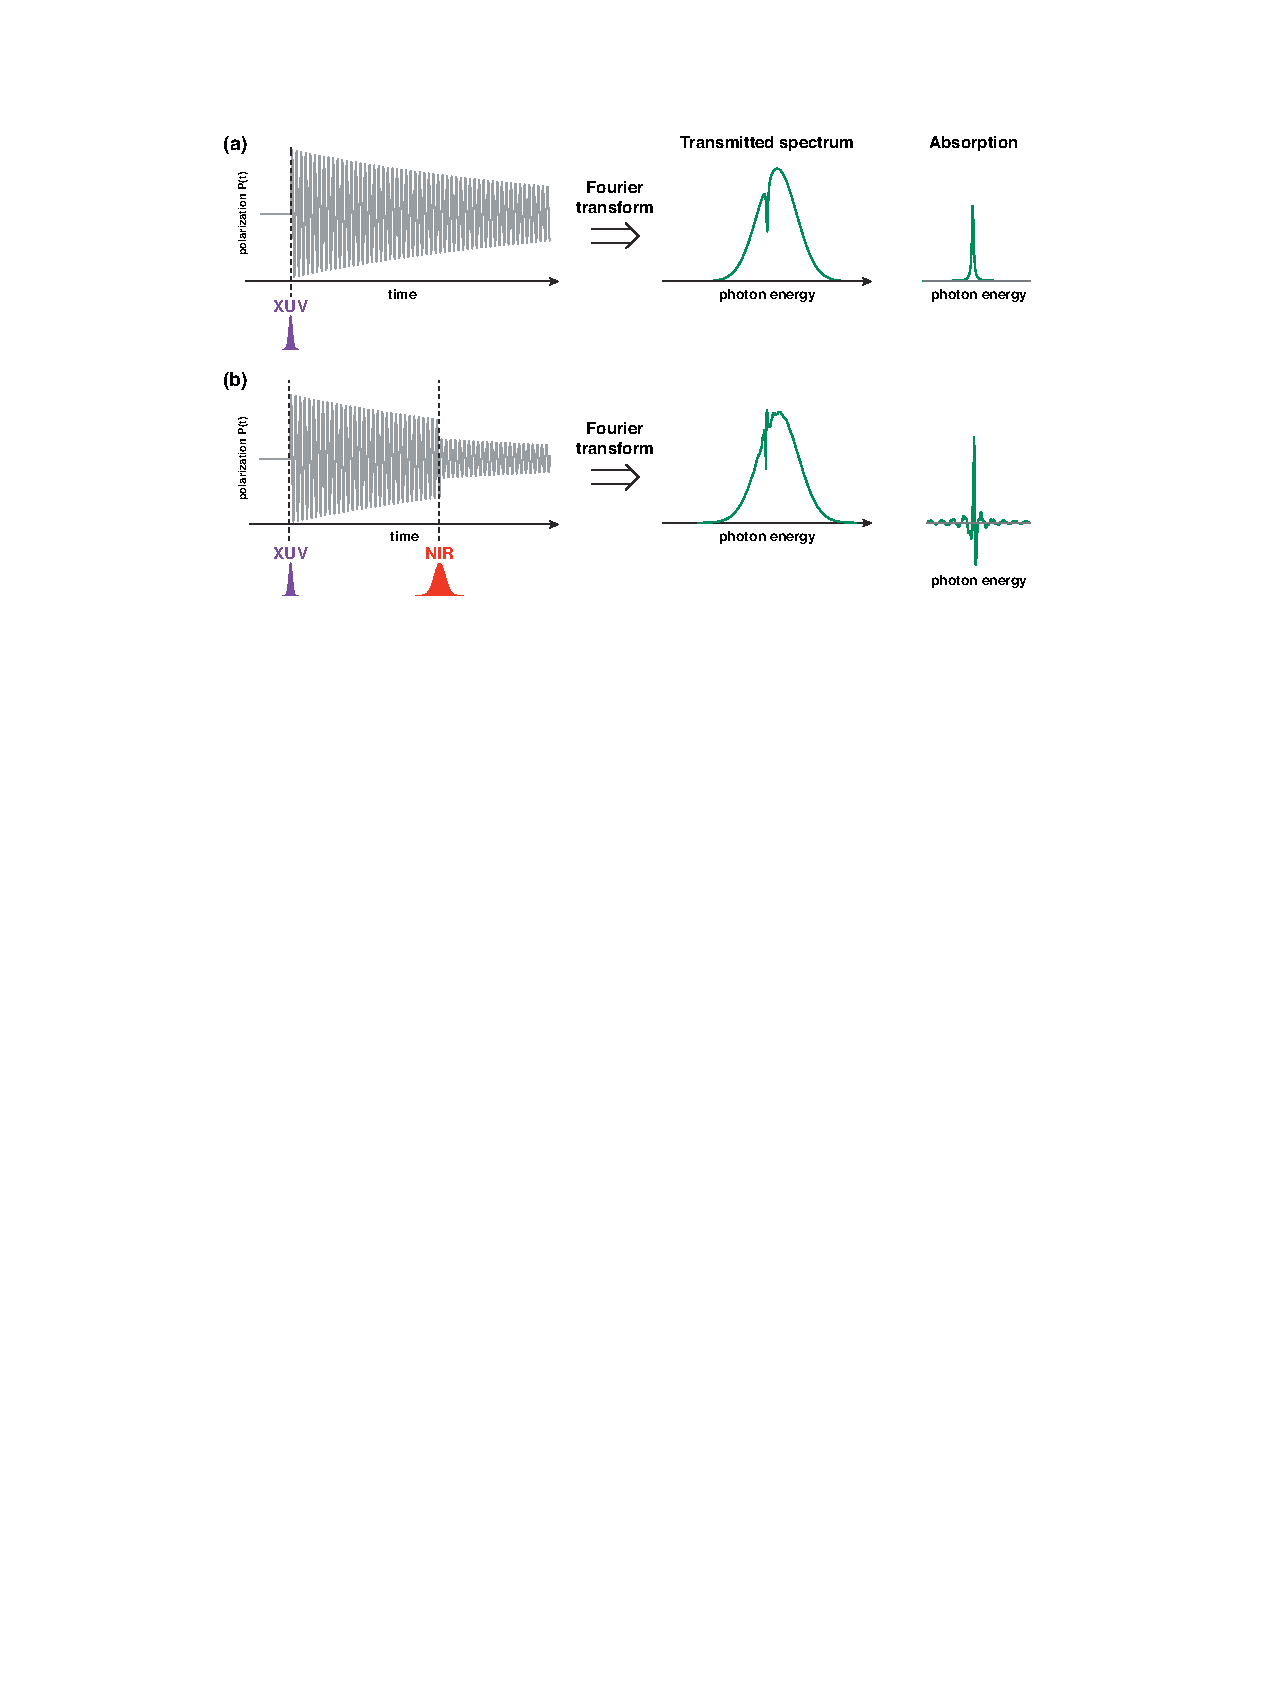
\includegraphics[width=1.0\textwidth]{figures/Introduction/gas_TA_sketch.pdf}
	\caption[Example electric field of XUV APT and its frequency spectrum]{(a) Example of the electric field of an XUV APT.  There is a burst every half-cycle of the fundamental field period $\tau_0$.  (b)  Spectral amplitude of APT.  Harmonics are separated by $2\omega_0=4\pi/\tau_0$.  Bandwidth of each harmonic is determined by the number of cycles in the fundamental pulse, and the overall bandwidth is determined by the pulse duration of each burst in the train. (b) Example of a two-color $\omega-2\omega$ fundamental field.  The asymmetry of the pulse means there is a burst once every cycle. (d) The spectral amplitude for the asymmetric field, and now there are even and odd harmonics.  The dashed line in (c) and (d) represent the spectral amplitude of just one of the pulses in the pulse train.}
	\label{fig:gas_TA_sketch}
\end{figure}

